%Dạng 1
\setcounter{ex}{0}
\section{Sự tương giao của hai đồ thị}
\subsection{Kiến thức cần nhớ}
\begin{khung}
	Cho hàm số $y=f(x)$ có đồ thị $(C_1)$ và hàm số $y=g(x)$ có đồ thị $(C_2)$.
	\begin{itemize}
		\item Số nghiệm của phương trình $f(x)=g(x)$ là số điểm chung của hai đồ thị $(C_1)$ và $(C_2)$.
		\item Phương trình $f(x)=g(x)$ được gọi là phương trình hoành độ giao điểm của hai đồ thị hàm số.
	\end{itemize}
\end{khung}
\subsection{Bài tập mẫu}
\Opensolutionfile{ans}[ans/ANS-DANG-31]
\begin{khung}
\begin{vd}[Đề tham khảo BGD 2022-2023]%[2D1B5-3]
	\immini{
		Cho hàm số bậc ba $y=f(x)$ có đồ thị là đường cong trong hình bên. Có bao nhiêu giá trị nguyên của tham số $m$ để phương trình $f(x)=m$ có ba nghiệm thực phân biệt?
		\choice
		{$2$}
		{$5$}
		{\True $3$}
		{$4$}
	}{
		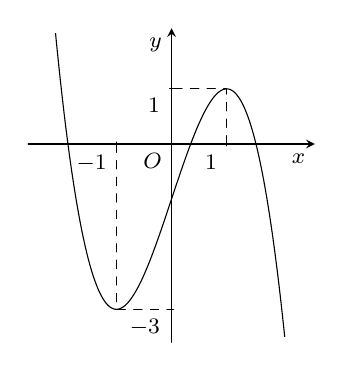
\begin{tikzpicture}[scale=0.7, font=\footnotesize, line join=round, line cap=round, >=stealth]
			\draw[->] (-2.6,0)--(2.6,0) node[below left] {$x$};
			\draw[->] (0,-3.6)--(0,2.1) node[below left] {$y$};
			\draw (0,0) node [below left] {$O$};
			\foreach \x in {-1,1}
			\draw[thin] (\x,1pt)--(\x,-1pt) node [below left] {$\x$};
			\foreach \y in {-3,1}
			\draw[thin] (1pt,\y)--(-1pt,\y) node [below left] {$\y$};
			\draw[dashed,thin](-1,0)--(-1,-3)--(0,-3);
			\draw[dashed,thin](1,0)--(1,1)--(0,1);
			\begin{scope}
				\clip (-2.5,-3.5) rectangle (2.5,2);
				\draw[samples=200,domain=-2.5:2.5,smooth,variable=\x] plot (\x,{-(\x^3)+3*(\x)-1});
			\end{scope}
		\end{tikzpicture}
	}
	\loigiai{
		Dựa vào đồ thị phương trình $f(x)=m$ có ba nghiệm thực phân biệt khi và chỉ khi $-3<m<1$.\\
		Kết hợp đề bài $m$ là giá trị nguyên suy ra $m\in \{-2;-1;0\}$.
	}
\end{vd}
\end{khung}
\subsection{Bài tập tương tự và phát triển}
\begin{ex}%[2D1B5-3]%Câu 1
		Cho hàm số $y=f(x)$ liên tục trên $\mathbb{R}$ có bảng biến thiên như sau
		\begin{center}
			
\begin{tikzpicture}
				\tkzTabInit[nocadre=false,lgt=1.2,espcl=2.5,deltacl=0.6]
				{$x$ /0.6,$y'$ /0.6,$y$ /2}
				{$-\infty$,$-1$,$0$,$1$,$+\infty$}
				\tkzTabLine{,-,$0$,+,$0$,-,$0$,+,}
				\tkzTabVar{+/$+\infty$, -/$\tfrac{1}{2}$,+/$5$,-/$\tfrac{1}{2}$,+/$+\infty$}
			\end{tikzpicture}
		\end{center}
		Số nghiệm thực phân biệt của phương trình $2f(x)-5=0$ là
		\choice
		{$3$}
		{$2$}
		{\True $4$}
		{$0$}
		\loigiai{
				Ta có $2 f(x)-5=0 \Leftrightarrow f(x)=\dfrac{5}{2}$.\\
				Số nghiệm thực của phương trình là số giao điểm của hai đồ thị hàm số $y=f(x)$ và $y=\dfrac{5}{2}$.\\
				Dựa vào bảng biến thiên ta thấy đường thẳng $y=\dfrac{5}{2}$ cắt đồ thị hàm số $y=f(x)$ tại $4$ điểm.\\
				Suy ra phương trình đã cho có $4$ nghiệm phân biệt.
			}
		\end{ex}
		
		
		
		\begin{ex}%[2D1B5-4]%Câu 3
			Đồ thị hàm số $y=x^3+2022x^2-2023x$ cắt trục hoành tại bao nhiêu điểm?
			\choice
			{$0$}
			{$2$}
			{$1$}
			{\True $3$}
			\loigiai{
				Phương trình hoành độ giao điểm đồ thị hàm số và trục hoành
				$$x^3+2022x^2-2023x=0 \Leftrightarrow \hoac{&x=0 \\ &x=1 \\ &x=-2023.}$$
				Vậy đồ thị hàm số cắt trục hoành tại $3$ điểm.
			}
		\end{ex}
		
		\begin{ex}%[2D1B5-4]%Câu 4
			Số giao điểm của đồ thị hàm số $y=x^3-3x+3$ và đường thẳng $y=x$.
			\choice
			{$2$}
			{\True $3$}
			{$1$}
			{$0$}
			\loigiai{
				Phương trình hoành độ giao điểm $x=x^3-3x+3 \Leftrightarrow x^3-4x+3=0 \Leftrightarrow \hoac{&x=1 \\ &x=\dfrac{-1 \pm \sqrt{13}}{2}.}$\\
				Vậy đồ thị hàm số $y=x^3-3x+3$ và đường thẳng $y=x$ có $3$ giao điểm.
			}
		\end{ex}
		
	
		\begin{ex}%[2D1B5-3]%Câu 7
		\immini{	Cho hàm số bậc ba $y=f(x)$ có đồ thị như hình vẽ bên. Số nghiệm của phương trình $3f(x)-4=0$ là
			\choice
			{\True $3$}
			{$1$}
			{$2$}
			{$0$}}{	\begin{tikzpicture}[scale=0.7,>=stealth, font=\footnotesize, line join=round, line cap=round]
				\def\a{1} \def\b{-3} \def\c{0} \def\d{4} % Hệ số
				\def\xmin{-2} \def\xmax{4}
				\def\ymin{-2} \def\ymax{5} 
				%	\draw[color=gray!50,dashed] (\xmin,\ymin) grid (\xmax,\ymax); 
				\draw[->] (\xmin,0)--(\xmax,0) node [below]{$x$};
				\draw[->] (0,\ymin)--(0,\ymax) node [left]{$y$};
				\node at (0,0) [below left]{$O$};
				\node at (-1,0) [below left]{$-1$};
				\node at (2,0) [below]{$2$};
				\node at (0,4) [above left]{$4$};
				\clip (\xmin+0.1,\ymin+0.1) rectangle (\xmax-0.5,\ymax-0.1);
				\draw[smooth,samples=300] plot(\x,{\a*(\x)^3+\b*(\x)^2+\c*(\x)+\d});
		\end{tikzpicture}}
			\loigiai{
			\immini{Ta có $3f(x)-4=0 \Leftrightarrow f(x)=\dfrac{4}{3}$.\\
				Số nghiệm thực của phương trình trên là số giao điểm của đồ thị hàm số $y=f(x)$ và đường thẳng $y=\dfrac{4}{3}$.\\
				Dựa vào đồ thị ta thấy đồ thị hàm số $y=f(x)$ và đường thẳng $y=\dfrac{4}{3}$ cắt nhau tại $3$ điểm.\\
				Vậy phương trình $3 f(x)-4=0$ có $3$ nghiệm.}{	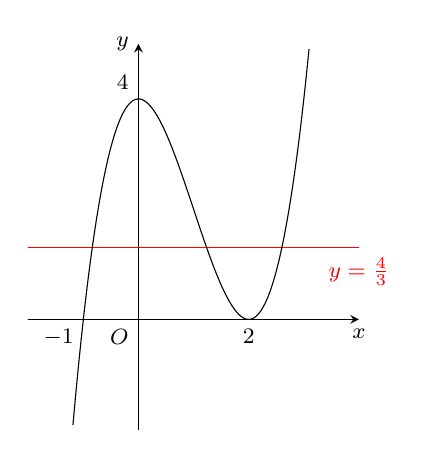
\begin{tikzpicture}[scale=0.7,>=stealth, font=\footnotesize, line join=round, line cap=round]
					\def\a{1} \def\b{-3} \def\c{0} \def\d{4} % Hệ số
					\def\xmin{-2} \def\xmax{4}
					\def\ymin{-2} \def\ymax{5} 
					%	\draw[color=gray!50,dashed] (\xmin,\ymin) grid (\xmax,\ymax); 
					\draw[->] (\xmin,0)--(\xmax,0) node [below]{$x$};
					\draw[->] (0,\ymin)--(0,\ymax) node [left]{$y$};
					\node at (0,0) [below left]{$O$};
					\node at (-1,0) [below left]{$-1$};
					\node at (2,0) [below]{$2$};
					\node at (0,4) [above left]{$4$};
					\draw[red] (-2,1.3)--(4,1.3) node [below]{$y=\frac{4}{3}$};
					\clip (\xmin+0.1,\ymin+0.1) rectangle (\xmax-0.5,\ymax-0.1);
					\draw[smooth,samples=300] plot(\x,{\a*(\x)^3+\b*(\x)^2+\c*(\x)+\d});
			\end{tikzpicture}}
			}
		\end{ex}
		
		\begin{ex}%[2D1B5-4]%Câu 8
			Cho hàm số $y=f(x)$ có đồ thị như hình vẽ.
			\begin{center}
				\begin{tikzpicture}[scale=1,>=stealth, font=\footnotesize, line join=round, line cap=round]
					\def\a{1} \def\b{-2} \def\c{0} % Hệ số
					\def\xmin{-3} \def\xmax{3}
					\def\ymin{-2} \def\ymax{3} 
					%	\draw[color=gray!50,dashed] (\xmin,\ymin) grid (\xmax,\ymax); 
					\draw[->] (\xmin,0)--(\xmax,0) node [below]{$x$};
					\draw[->] (0,\ymin)--(0,\ymax) node [left]{$y$};
					\node at (0,0) [above left]{$O$};
					\clip (\xmin+0.1,\ymin+0.1) rectangle (\xmax-0.5,\ymax-0.1);
					\draw[smooth,samples=300] plot(\x,{\a*(\x)^4+\b*(\x)^2+\c});
				\end{tikzpicture}
			\end{center}
			Số nghiệm thực của phương trình $f(x)=3$ là
			\choice
			{$3$}
			{$1$}
			{\True $2$}
			{$0$}
			\loigiai{
				Số nghiệm thực của phương trình $f(x)=3$ bằng số giao điểm của đồ thị hàm số $y=f(x)$ và đường thẳng $y=3$.\\
				Ta có đường thẳng $y=3$ song song với trục hoành và cắt trục tung tại điểm có tọa độ $(0;3)$.\\
				Từ đồ thị ta thấy đường thẳng $y=3$ cắt đồ thị hàm số $y=f(x)$ tại hai điểm phân biệt.\\
				Do đó phương trình $f(x)=3$ có $2$ nghiệm thực phân biệt.
			}
		\end{ex}
		
		\begin{ex}%[2D1B5-4]%Câu 9
			Đồ thị hàm số $y=\dfrac{x+5}{x-1}$ cắt trục hoành tại điểm có hoành độ bằng
			\choice
			{\True $x=-5$}
			{$x=5$}
			{$x=-1$}
			{$x=1$}
			\loigiai{
			Ta có $y=0 \Leftrightarrow x=-5$.}
		\end{ex}
		
		\begin{ex}%[2D1B5-4]%Câu 10
			Số giao điểm của đồ thị hàm số $y=\dfrac{3 x+1}{x-3}$ và đường thẳng $y=3$ là
			\choice
			{ $3$}
			{$1$}
			{$2$}
			{\True $0$}
			\loigiai{
				Xét phương trình hoành độ giao điểm $\dfrac{3 x+1}{x-3}=3 \Leftrightarrow \heva{&3x+1=3x-9\, (\text{vô nghiệm})\\ &x \neq 3.}$.\\
				Vậy đồ thị hàm số $y=\dfrac{3x+1}{x-3}$ và đường thẳng $y=3$ không có điểm chung.
			}
		\end{ex}
		
		\begin{ex}%[2D1B5-4]%Câu 11
			Số giao điểm của đồ thị hàm số $y=x^3-x$ với trục hoành là
			\choice
			{$2$}
			{$0$}
			{\True $3$}
			{$1$}
			\loigiai{
				Phương trình hoành độ giao điểm là $x^3-x=0 \Leftrightarrow \hoac{&x=0 \\ &x= \pm 1.}$\\
				Vậy đồ thị hàm số cắt trục hành tại ba điểm phân biệt.
			}
		\end{ex}
		
		\begin{ex}%[2D1B5-4]%Câu 12
			Số giao điểm của đồ thị hàm số $y=3x^3-6x^2+8x-5$ và trục hoành.
			\choice
			{\True $1$}
			{$2$}
			{$0$}
			{$3$}
			\loigiai{
				Phương trình hoành độ giao điểm của đồ thị hàm số $y=3x^3-6x^2+8 x-5$ với trục hoành
				$$
				3x^3-6x^2+8x-5=0 \Leftrightarrow (x-1)\left(3x^2-3x+5\right)=0 \Leftrightarrow \hoac{&x-1=0\\ &3x^2-3x+5=0} \Leftrightarrow \hoac{&x=1 \\ &3x^2-3x+5=0.}
				$$
				Do phương trình $3x^2-3x+5=0$ có $\Delta =(-3)^2-4\cdot 3\cdot 5=-51<0$ suy ra phương trình vô nghiệm nên đồ thị hàm số $y=3x^3-6x^2+8x-5$ cắt trục hoành tại đúng một điểm.
			}
		\end{ex}
		
		\begin{ex}%[2D1B5-3]%Câu 13
			Cho hàm số $y=f(x)$ có bảng biến thiên như hình vẽ. Hỏi phương trình $3f(x)-4=0$ có tất cả bao nhiêu nghiệm thực?
		\begin{center}
			
\begin{tikzpicture}
				\tikzset{double style/.append style={double distance=1.5pt}}
				\tkzTabInit[lgt=1.2,espcl=2.5,deltacl=0.6]
				{$x$ /0.6,$y$ /2}
				{$-\infty$,$0$,$+\infty$}
				%\tkzTabLine{,+,d,+,}
				\tkzTabVar{+/$+\infty$,-D-/$1$/$2$,+/$+\infty$}
			\end{tikzpicture}
		\end{center}
			\choice
			{$3$}
			{$0$}
			{\True $1$}
			{$2$}
			\loigiai{
				Ta có $3 f(x)-4=0 \Leftrightarrow f(x)=\dfrac{4}{3}$.\\		
				Dựa vào bảng biến thiên phương trình trên có $1$ nghiệm duy nhất.
			}
		\end{ex}
		
		\begin{ex}%[2D1B5-3]%Câu 14
			Cho hàm số $f(x)$ có bảng biến thiên như sau
			\begin{center}
				
\begin{tikzpicture}
					\tkzTabInit[lgt=1.2,espcl=2.5,deltacl=0.6]
					{$x$ /0.6,$y'$ /0.6,$y$ /2}
					{$-\infty$,$-1$,$0$,$1$,$+\infty$}
					\tkzTabLine{,-,$0$,+,$0$,-,$0$,+,}
					\tkzTabVar{+/$+\infty$, -/$-4$,+/$-3$,-/$-4$,+/$+\infty$}
				\end{tikzpicture}
			\end{center}
			Số nghiệm thực của phương trình $f(x)+5=0$ là
			\choice
			{$2$}
			{$3$}
			{$1$}
			{\True $0$}
			\loigiai{
				Phương trình đã cho tương đương với $f(x)=-5$.\\
				Ta thấy đường thẳng $y=-5$ không có điểm chung với đồ thị hàm số $y=f(x)$ nên phương trình đã cho vô nghiệm.
			}
		\end{ex}
		
		\begin{ex}%[2D1B5-3]%Câu 15
			Cho hàm số $y=f(x)$ có bảng biến thiên sau
			\begin{center}
				
\begin{tikzpicture}
					\tkzTabInit[lgt=1.2,espcl=2.5,deltacl=0.6]
					{$x$ /0.6, $y'$ /0.6, $y$ /2.5}
					{$-\infty$,$0$,$4$,$+\infty$}
					\tkzTabLine{,+,$0$,-,$0$,+,}
					\tkzTabVar{-/$-\infty$,+/$3$,-/$-5$,+/$+\infty$}
				\end{tikzpicture}
			\end{center}
			Phương trình $f(x)=2$ có bao nhiêu nghiệm?
			\choice
			{$2$}
			{$4$}
			{$1$}
			{\True $3$}
			\loigiai{
				Xét sự tương giao giữa đồ thị $y=f(x)$ và đường thẳng $y=2$, ta thấy đường thẳng $y=2$ cắt đồ thị $y=f(x)$ tại $3$ điểm phân biệt.\\
				Do đó phương trình $f(x)=2$ có $3$ nghiệm.
			}
		\end{ex}
		
		\begin{ex}%[2D1B5-4]%Câu 16
			Đồ thị của hàm số $y=x^3+2x^2-x+1$ và đồ thị của hàm số $y=x^2-x+3$ có bao nhiêu điểm chung?
			\choice
			{$2$}
			{\True$1$}
			{$3$}
			{$0$}
			\loigiai{
				Xét phương trình hoành độ giao điểm $x^3+2x^2-x+1=x^2-x+3\quad (\ast)$.\\
				Khi đó, phương trình tương đương
				$$x^3+x^2-2=0 \Leftrightarrow(x-1)\left(x^2+2x+2\right)=0 \Leftrightarrow x=1.$$
				Vậy phương trình $(\ast)$ có một nghiệm suy ra đồ thị của hai hàm số đã cho có một điểm chung.
			}
		\end{ex}
		
		\begin{ex}%[2D1B5-4]%Câu 17
			Số giao điểm của đồ thị hàm số $y=(x-3)\left(x^2+x+4\right)$ với trục hoành là
			\choice
			{$2$}
			{$0$}
			{\True $1$}
			{ $3$}
			\loigiai{
				Số giao điểm của đồ thị hàm số $y=(x-3)\left(x^2+x+4\right)$ với trục hoành bằng số nghiệm của phương trình
				$$
				\begin{aligned}
					& (x-3)\left(x^2+x+4\right)=0 \\
					& \Leftrightarrow x-3=0\left(x^2+x+4>0, \forall x \in \mathbb{R}\right) \\
					& \Leftrightarrow x=3 .
				\end{aligned}
				$$}
		\end{ex}
		
		
		\begin{ex}%[2D1B5-3]%Câu 19
			\immini{
			Cho hàm bậc ba $y=f(x)$ có đồ thị như hình vẽ. Số nghiệm của phương trình $f(x)=2$ là
			\choice
			{\True $2$}
			{$0$}
			{$3$}
			{$1$}
		}
		{
			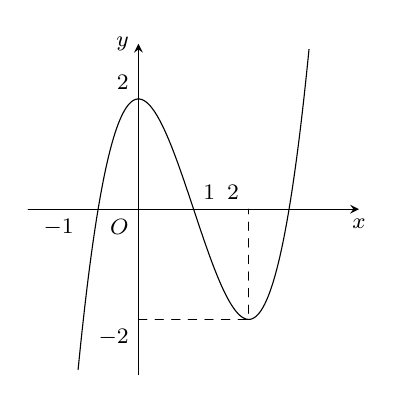
\begin{tikzpicture}[scale=0.7,>=stealth, font=\footnotesize, line join=round, line cap=round]
				\def\a{1} \def\b{-3} \def\c{0} \def\d{2} % Hệ số
				\def\xmin{-2} \def\xmax{4}
				\def\ymin{-3} \def\ymax{3} 
				%\draw[color=gray!50,dashed] (\xmin,\ymin) grid (\xmax,\ymax); 
				\draw[->] (\xmin,0)--(\xmax,0) node [below]{$x$};
				\draw[->] (0,\ymin)--(0,\ymax) node [left]{$y$};
				\node at (0,0) [below left]{$O$};
				\node at (-1,0) [below left]{$-1$};
				\node at (1,0) [above right]{$1$};
				\node at (2,0) [above left]{$2$};
				\node at (0,2) [above left]{$2$};
				\node at (0,-2) [below left]{$-2$};
				\draw[dashed] (0,-2)--(2,-2)--(2,0);
				%\draw[red] (-2,2)--(4,2);
				%\node at (1,2.2) [above right]{$y=2$};
				\clip (\xmin+0.1,\ymin+0.1) rectangle (\xmax-0.5,\ymax-0.1);
				\draw[smooth,samples=300] plot(\x,{\a*(\x)^3+\b*(\x)^2+\c*(\x)+\d});
			\end{tikzpicture}
		
		}
		\loigiai{
		\immini{Vẽ đường thẳng $y=2$ ta thấy đường thẳng $y=2$ cắt đồ thị hàm số $y=f(x)$ tại hai điểm.\\
		Do đó số nghiệm của phương trình $f(x)=2$ là $2$.}{	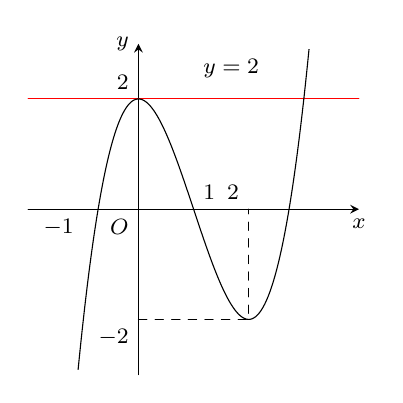
\begin{tikzpicture}[scale=0.7,>=stealth, font=\footnotesize, line join=round, line cap=round]
			\def\a{1} \def\b{-3} \def\c{0} \def\d{2} % Hệ số
			\def\xmin{-2} \def\xmax{4}
			\def\ymin{-3} \def\ymax{3} 
			%\draw[color=gray!50,dashed] (\xmin,\ymin) grid (\xmax,\ymax); 
			\draw[->] (\xmin,0)--(\xmax,0) node [below]{$x$};
			\draw[->] (0,\ymin)--(0,\ymax) node [left]{$y$};
			\node at (0,0) [below left]{$O$};
			\node at (-1,0) [below left]{$-1$};
			\node at (1,0) [above right]{$1$};
			\node at (2,0) [above left]{$2$};
			\node at (0,2) [above left]{$2$};
			\node at (0,-2) [below left]{$-2$};
			\draw[dashed] (0,-2)--(2,-2)--(2,0);
			\draw[red] (-2,2)--(4,2);
			\node at (1,2.2) [above right]{$y=2$};
			\clip (\xmin+0.1,\ymin+0.1) rectangle (\xmax-0.5,\ymax-0.1);
			\draw[smooth,samples=300] plot(\x,{\a*(\x)^3+\b*(\x)^2+\c*(\x)+\d});
	\end{tikzpicture}}
	}
		\end{ex}
	
		\begin{ex}%[2-2021-DTK-05]%[2D1B5-3]
			\immini{Cho hàm số bậc bốn $y=f(x)$ có đồ thị như hình vẽ bên. Số nghiệm của phương trình $f(x)+1=0$ là
				\choice
				{$2$}
				{$3$}
				{\True $4$}
				{$1$}
			}{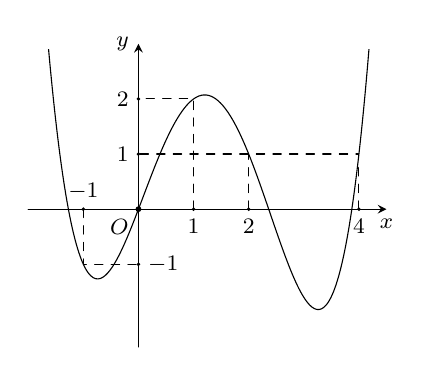
\begin{tikzpicture}[line join = round, line cap = round,>=stealth,font=\footnotesize,scale=0.7]
					\def\xt{-2} \def\xp{4.5} \def\yd{-2.5} \def\yt{3}
					\def\a{0.225}
					\def\b{-1.116666}
					\def\c{0.275}
					\def\d{2.6166666}
					\def\e{0}
					\draw[->] (\xt,0)--(\xp,0) node[below]{$x$};
					\draw[->] (0,\yd)--(0,\yt) node[left]{$y$};
					\fill (0,0) circle (1.5pt) node[below left]{$O$};
					\draw[dashed](-1,0)--(-1,-1)--(0,-1);
					\draw[dashed](1,0)--(1,2)--(0,2);
					\draw[dashed](2,0)--(2,1);
					\draw[dashed](4,0)--(4,1)--(0,1);
					\fill (0,-1) circle (1pt) node[ right ]{$-1$};
					\fill (0,1) circle (1pt) node[ left ]{$1$};
					\fill (0,2) circle (1pt) node[ left ]{$2$};
					\fill (-1,0) circle (1pt) node[above]{$-1$};
					\fill (1,0) circle (1pt) node[below]{$1$};
					\fill (2,0) circle (1pt) node[below]{$2$};
					\fill (4,0) circle (1pt) node[below]{$4$};
					\begin{scope}
						\clip (\xt+0.1,\yd+0.1) rectangle (\xp-0.1,\yt-0.1);
						\draw[samples=150,smooth,domain=\xt:\xp] plot(\x,{\a*(\x)^4+(\b)*(\x)^3+(\c)*(\x)^2+\d*(\x)+\e});
					\end{scope}
			\end{tikzpicture}}
			\loigiai{
				\immini{Ta có $f(x)+1=0\Leftrightarrow f(x)=-1$. \\
					Số nghiệm của phương trình $f(x)+1=0$ là số giao điểm của đồ thị hàm số $y=f(x)$ và $y=-1$.\\
					Dựa vào đồ thị ta thấy đường thẳng $y=-1$ cắt đồ thị hàm số $y=f(x)$ tại $4$ điểm phân biệt nên phương trình đã cho có $4$ nghiệm.
				}{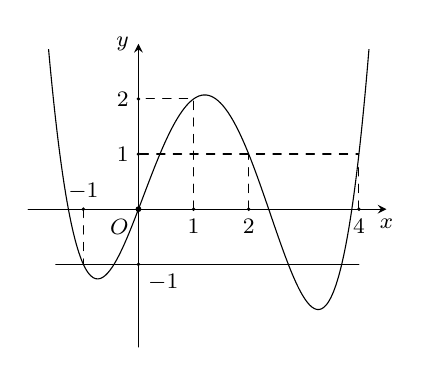
\begin{tikzpicture}[line join = round, line cap = round,>=stealth,font=\footnotesize,scale=0.7]
						\def\xt{-2} \def\xp{4.5} \def\yd{-2.5} \def\yt{3}
						\def\a{0.225}
						\def\b{-1.116666}
						\def\c{0.275}
						\def\d{2.6166666}
						\def\e{0}
						\draw[->] (\xt,0)--(\xp,0) node[below]{$x$};
						\draw[->] (0,\yd)--(0,\yt) node[left]{$y$};
						\fill (0,0) circle (1.5pt) node[below left]{$O$};
						\draw[dashed](-1,0)--(-1,-1)--(0,-1);
						\draw[dashed](1,0)--(1,2)--(0,2);
						\draw[dashed](2,0)--(2,1);
						\draw[dashed](4,0)--(4,1)--(0,1);
						\draw (-1.5,-1)--(4,-1);
						\fill (0,-1) circle (1pt) node[below right ]{$-1$};
						\fill (0,1) circle (1pt) node[ left ]{$1$};
						\fill (0,2) circle (1pt) node[ left ]{$2$};
						\fill (-1,0) circle (1pt) node[above]{$-1$};
						\fill (1,0) circle (1pt) node[below]{$1$};
						\fill (2,0) circle (1pt) node[below]{$2$};
						\fill (4,0) circle (1pt) node[below]{$4$};
						\begin{scope}
							\clip (\xt+0.1,\yd+0.1) rectangle (\xp-0.1,\yt-0.1);
							\draw[samples=150,smooth,domain=\xt:\xp] plot(\x,{\a*(\x)^4+(\b)*(\x)^3+(\c)*(\x)^2+\d*(\x)+\e});
						\end{scope}
				\end{tikzpicture}}
			}
		\end{ex}
	
		\begin{ex}%[2D1B5-3]%Câu 20
			Cho hàm số $y=f(x)$ có bảng biến thiên như sau
			\begin{center}
					
\begin{tikzpicture}
						\tkzTabInit[lgt=1.2,espcl=2.5,deltacl=0.6]
						{$x$ /0.6,$y'$ /0.6,$y$ /2}
						{$-\infty$,$-2$,$0$,$2$,$+\infty$}
						\tkzTabLine{,-,$0$,+,$0$,-,$0$,+,}
						\tkzTabVar{+/$+\infty$, -/$-2$,+/$1$,-/$-2$,+/$+\infty$}
					\end{tikzpicture}
			\end{center}
			Số nghiệm thực của phương trình $2f(x)+3=0$ là
			\choice
			{$2$}
			{\True $4$}
			{$3$}
			{$6$}
			\loigiai{
				Ta có $2f(x)+3=0 \Leftrightarrow f(x)=-\dfrac{3}{2}$.\\
				Dựa vào bảng biến thiên, phương trình $f(x)=-\dfrac{3}{2}$ có $4$ nghiệm thực.
			}
		\end{ex}
	
	\begin{ex}%[2D1B5-3]
		Cho hàm số $y=f(x)$ xác định, liên tục trên $\mathbb{R}$ và có bảng biến thiên như hình vẽ
		\begin{center}	
			\begin{tikzpicture}[scale=1,font=\footnotesize,line join=round,line cap=round,>=stealth]
				\tkzTabInit[nocadre=false,lgt=1.2,espcl=2.5,deltacl=0.6]{$x$/.6 ,$y'$/.6,$y$/2}
				{$-\infty$ , $-\sqrt{2}$ ,$0$ ,$\sqrt{2}$ ,  $+\infty$}
				\tkzTabLine{ , - , 0 ,+ , 0 , - , 0 , + ,}
				\path
				(N12)node[below right](A){$+\infty$}
				(N23)node[above](B){$-4$}
				(N32)node[below](C){$0$}
				(N43)node[above ](D){$-4$}
				(N52)node[below](E){$+\infty$}
				;
				\draw[->] (A)--(B);
				\draw[->] (B)--(C);
				\draw[->] (C)--(D);
				\draw[->] (D)--(E);
			\end{tikzpicture}
		\end{center}
		Tìm $m$ để phương trình $f(x)+3=m$ vô nghiệm.	
		\choice
		{$m>-1$}
		{$m\geq -4$}
		{$m\leq -4$}
		{\True $m<-1$}
		\loigiai{
			Ta có $f(x)+3=m \Leftrightarrow f(x)=m-3$.\\
			Theo bảng biến thiên, phương trình vô nghiệm khi và chỉ khi $m-3<-4 \Leftrightarrow m<-1$.	
		}
	\end{ex}
\begin{ex}%[2D1B5-3]
	\immini{
		Cho hàm số $y=f(x)$ có đồ thị là hình bên. Phương trình $4-3f(x)=0$ có bao nhiêu nghiệm?
		\choice
		{$1$}
		{\True $3$}
		{$2$}
		{$0$}}
	{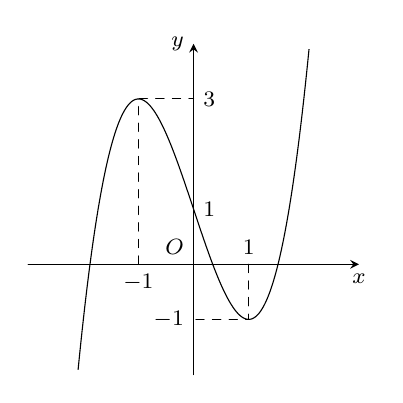
\begin{tikzpicture}[scale=.7,>=stealth, font=\footnotesize, line join=round, line cap=round]
			\def\a{1} \def\b{0} \def\c{-3} \def\d{1} % Hệ số
			\def\xmin{-3} \def\xmax{3}
			\def\ymin{-2} \def\ymax{4}
			%		\draw[color=gray!50,dashed] (\xmin,\ymin) grid (\xmax,\ymax);
			\draw[->] (\xmin,0)--(\xmax,0) node [below]{$x$};
			\draw[->] (0,\ymin)--(0,\ymax) node [left]{$y$};
			\node at (0,0) [above left]{$O$};
			\node at (0,1) [right]{$1$};
			\node at (0,3) [right]{$3$};
			\node at (0,-1) [left]{$-1$};
			\node at (1,0) [above]{$1$};
			\node at (-1,0) [below]{$-1$};
			\draw[dashed] (1,0)--(1,-1)--(0,-1);
			\draw[dashed] (-1,0)--(-1,3)--(0,3);
			\clip (\xmin+0.1,\ymin+0.1) rectangle (\xmax-0.5,\ymax-0.1);
			\draw[smooth,samples=300] plot(\x,{\a*(\x)^3+\b*(\x)^2+\c*(\x)+\d});
	\end{tikzpicture}}
	\loigiai{
		\immini
		{Ta có $4-3f(x)=0 \Leftrightarrow f(x)=\dfrac{4}{3}$.\\
			Do đường thẳng $y=\dfrac{4}{3}$ cắt đồ thị tại $3$ điểm phân biệt nên phương trình $4-3f(x)=0$ có $3$ nghiệm.}
		{\begin{tikzpicture}[scale=.7,>=stealth, font=\footnotesize, line join=round, line cap=round]
				\def\a{1} \def\b{0} \def\c{-3} \def\d{1} % Hệ số
				\def\xmin{-3} \def\xmax{3}
				\def\ymin{-2} \def\ymax{4}
				%\draw[color=gray!50,dashed] (\xmin,\ymin) grid (\xmax,\ymax);
				\draw[->] (\xmin,0)--(\xmax,0) node [below]{$x$};
				\draw[->] (0,\ymin)--(0,\ymax) node [left]{$y$};
				\node at (0,0) [above left]{$O$};
				\node at (0,1) [right]{$1$};
				\node at (0,3) [right]{$3$};
				\node at (0,-1) [left]{$-1$};
				\node at (1,0) [above]{$1$};
				\node at (-1,0) [below]{$-1$};
				\node at (3,1.33) [right]{$y=\dfrac{4}{3}$};
				\draw[dashed] (1,0)--(1,-1)--(0,-1);
				\draw[dashed] (-1,0)--(-1,3)--(0,3);
				\draw (-3,1.33)--(3,1.33);
				\clip (\xmin+0.1,\ymin+0.1) rectangle (\xmax-0.5,\ymax-0.1);
				\draw[smooth,samples=300] plot(\x,{\a*(\x)^3+\b*(\x)^2+\c*(\x)+\d});
		\end{tikzpicture}}
	}
\end{ex}


\begin{ex}%[2D1B5-3]
	Cho hàm số $y=f(x)$ có bảng biến thiên như sau
	\begin{center}
		
\begin{tikzpicture}[scale=0.7, font=\footnotesize, line join=round, line cap=round, >=stealth]
			\tkzTabInit[nocadre=false,lgt=1.2,espcl=2.5,deltacl=0.6]{$x$ /.8,$f'(x)$ /.8, $f(x)$ /2}{$-\infty$,$-1$,$2$,$+\infty$}
			\tkzTabLine{,-,0,+,0,-,}
			\tkzTabVar{+/ $+\infty$ , -/$-2$,+/ $2$, -/$-\infty$}
		\end{tikzpicture}
	\end{center}
	Số nghiệm của phương trình $2f(x)-5=0$ là
	\choice
	{$2$}
	{\True $1$}
	{$3$}
	{$0$}
	\loigiai{
		Ta có $2f(x)-5=0\Leftrightarrow f(x)=\dfrac{5}{2}$.\\
		Theo bảng biến thiên đường thẳng $y=\dfrac{5}{2}$ cắt đồ thị tại $1$ điểm nên phương trình $2f(x)-5=0$ có $1$ nghiệm.
	}
\end{ex}
\Closesolutionfile{ans}
%======================
\subsection{Bảng đáp án}
\inputansbox{8}{ans/ANS-DANG-31}

